%!TEX TS-program = ../make.zsh

\begin{frame}{Flasher-simulation example}

  Calibration: Find out the properties of the hole ice by comparing simulations with differnt properties to data of IceCube's LED-flasher-calibration system.\\

  \centering
  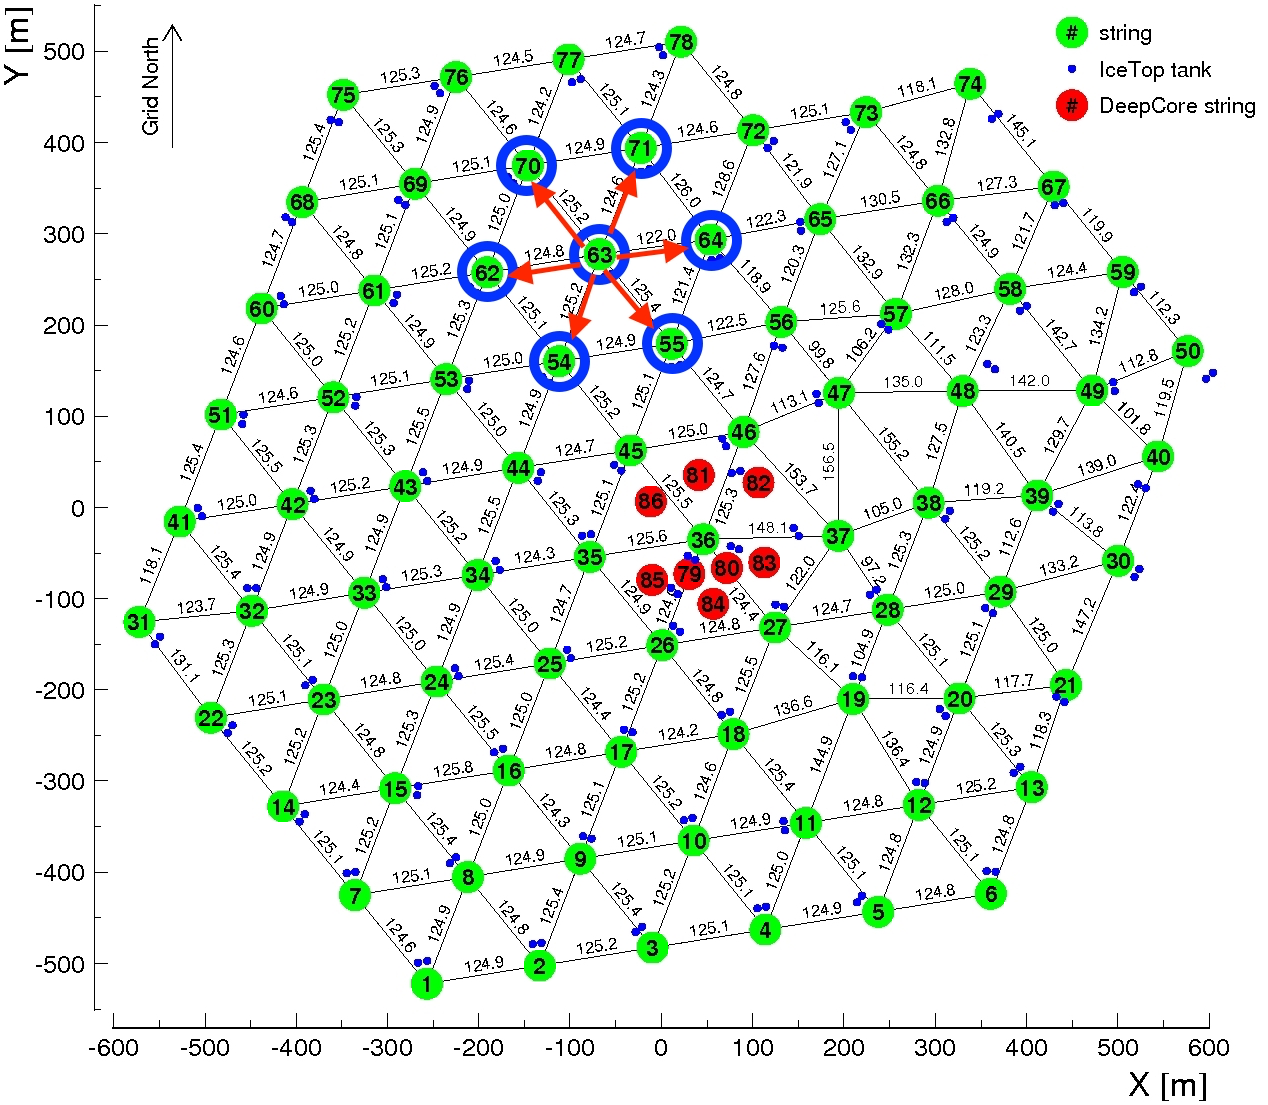
\includegraphics[height=0.35\textheight]{img/flasher-scenario}\hspace{1.2cm}
  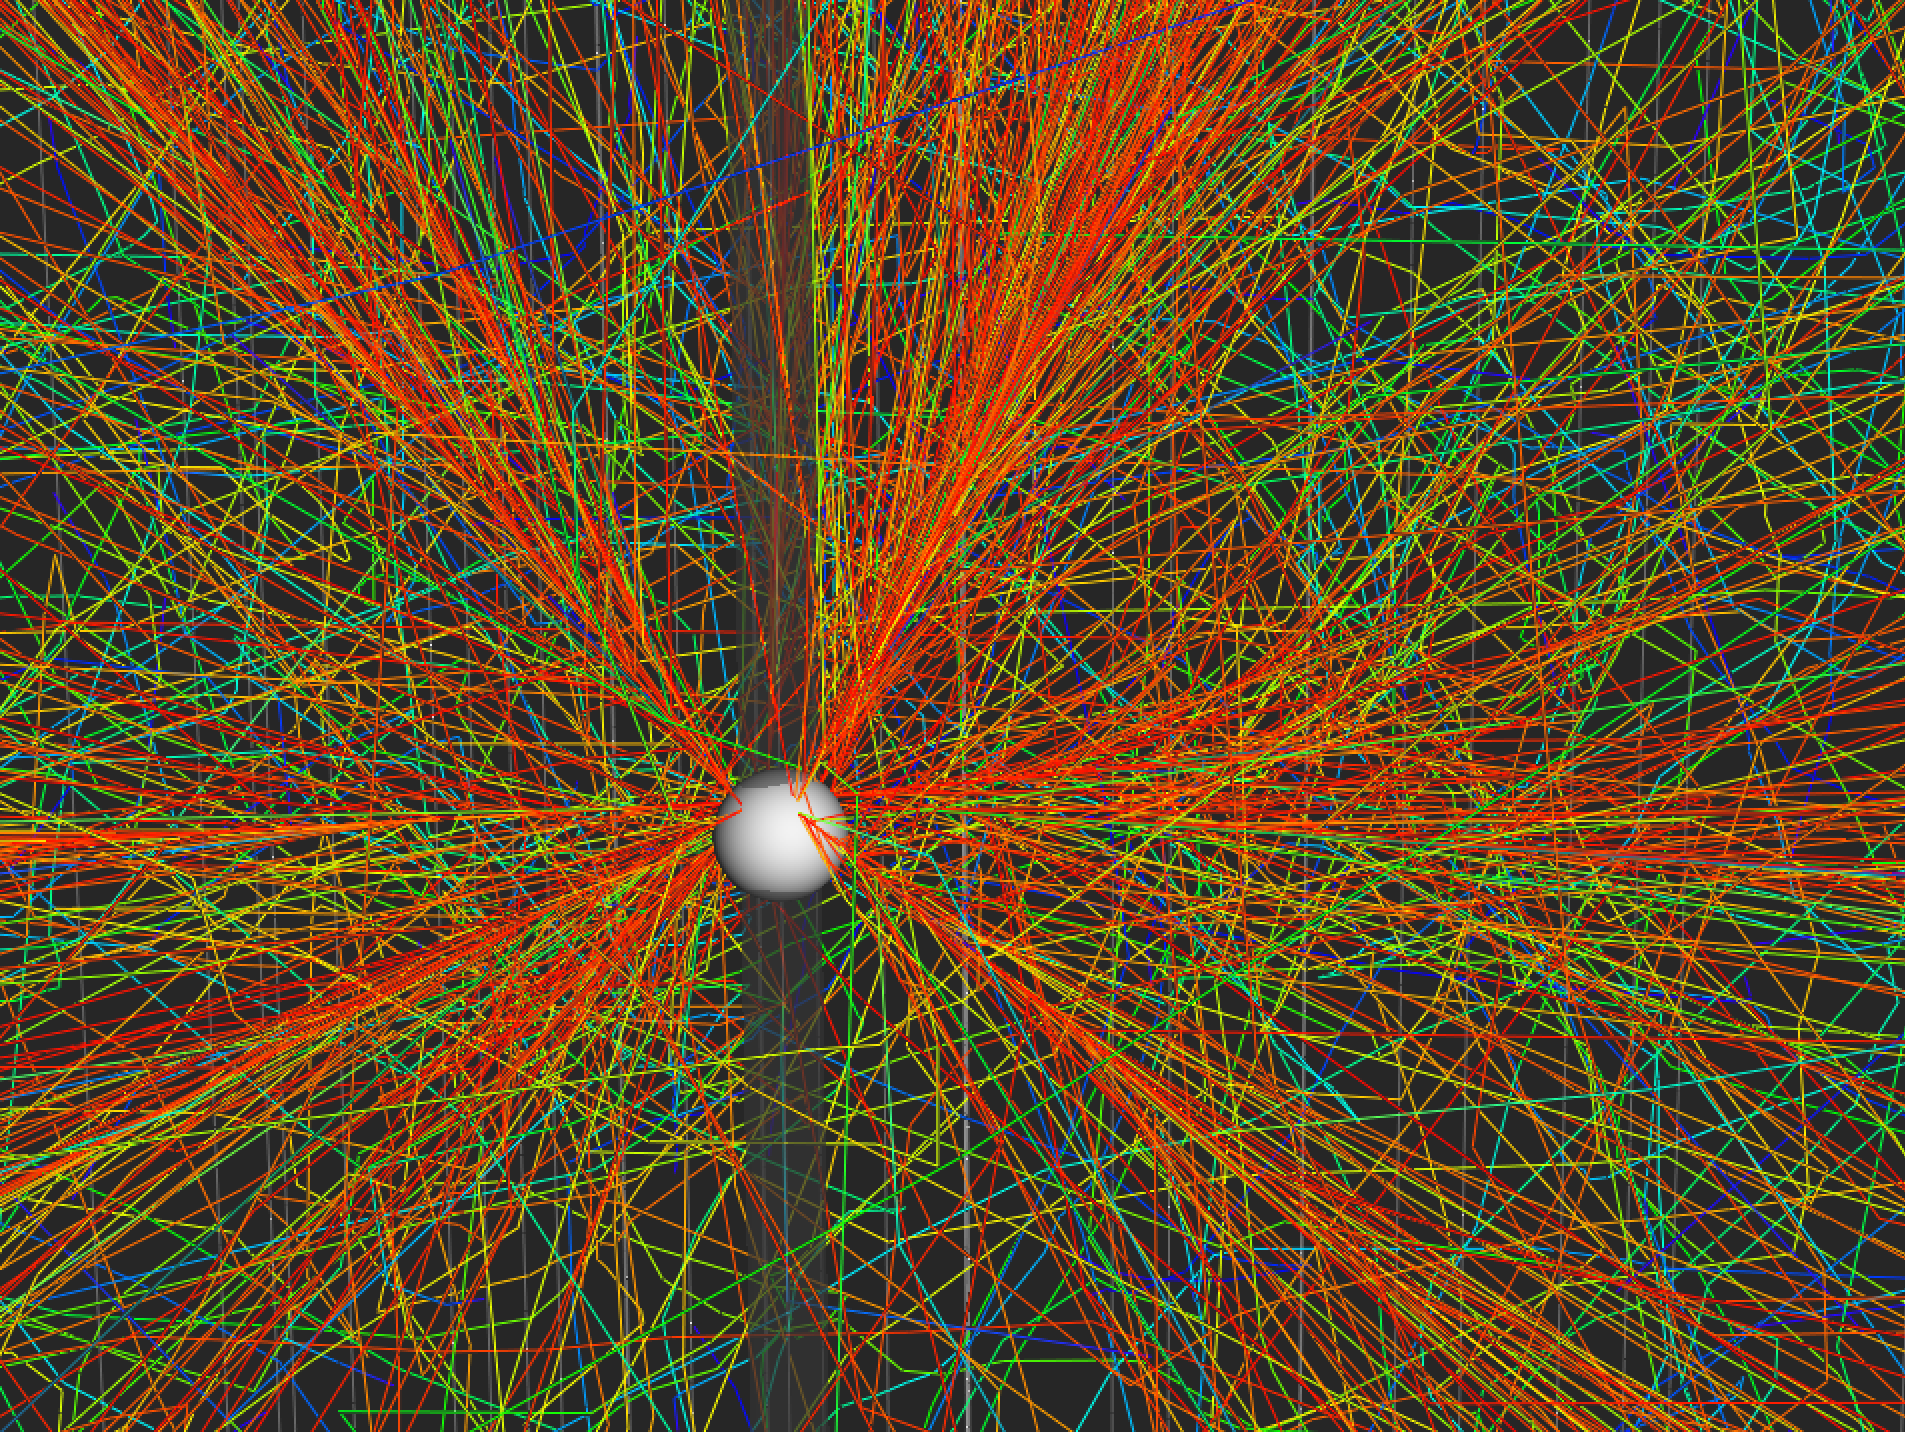
\includegraphics[height=0.35\textheight]{img/flasher-steamshovel-sending}

  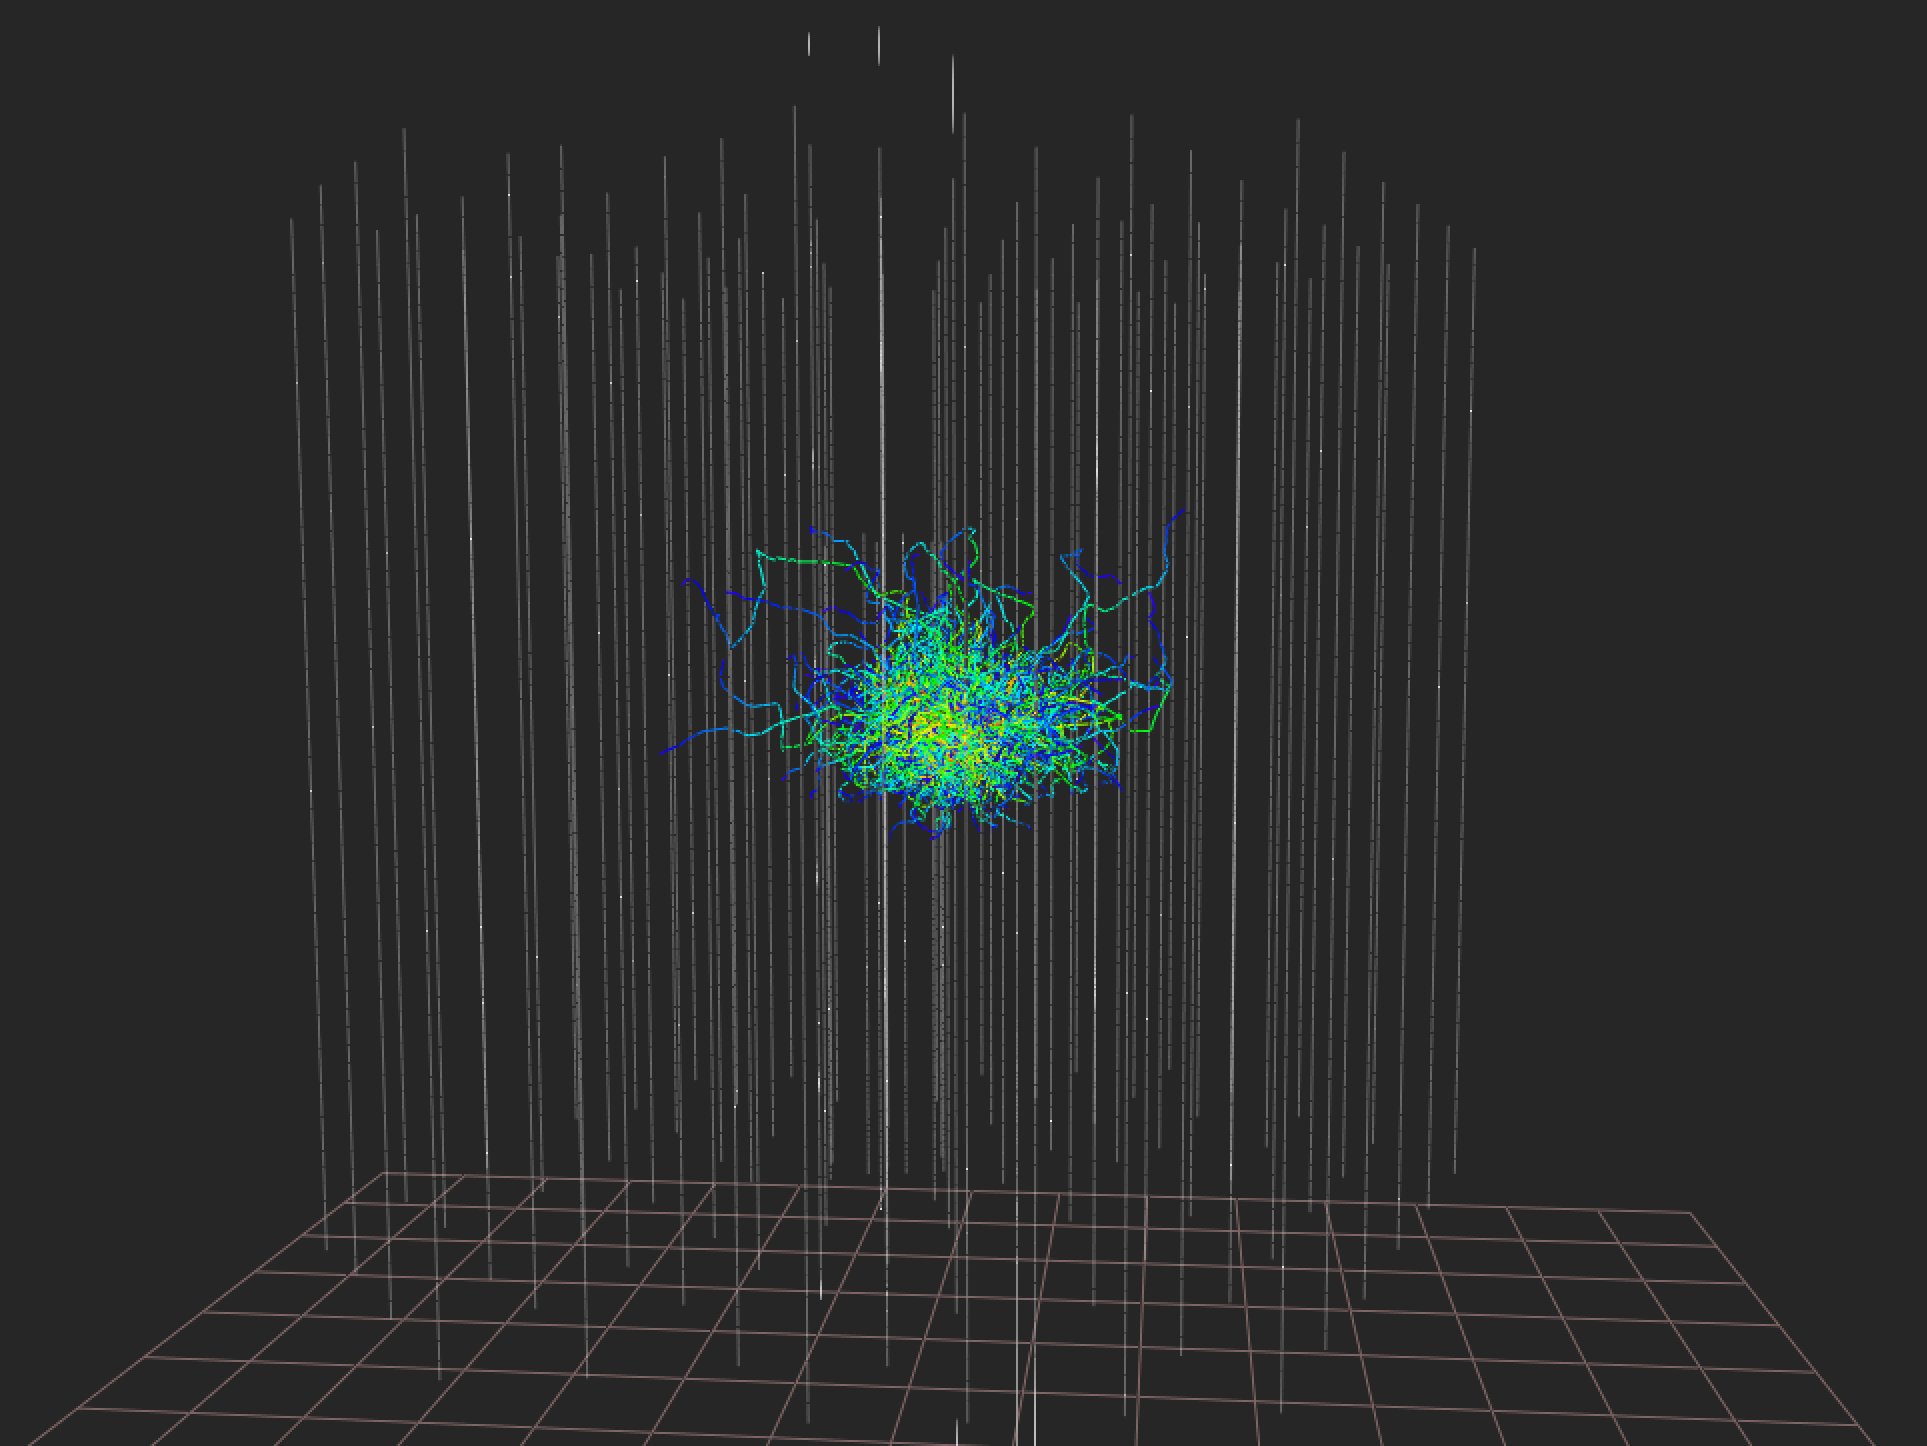
\includegraphics[height=0.35\textheight]{img/flasher-steamshovel-total}\hspace{3mm}
  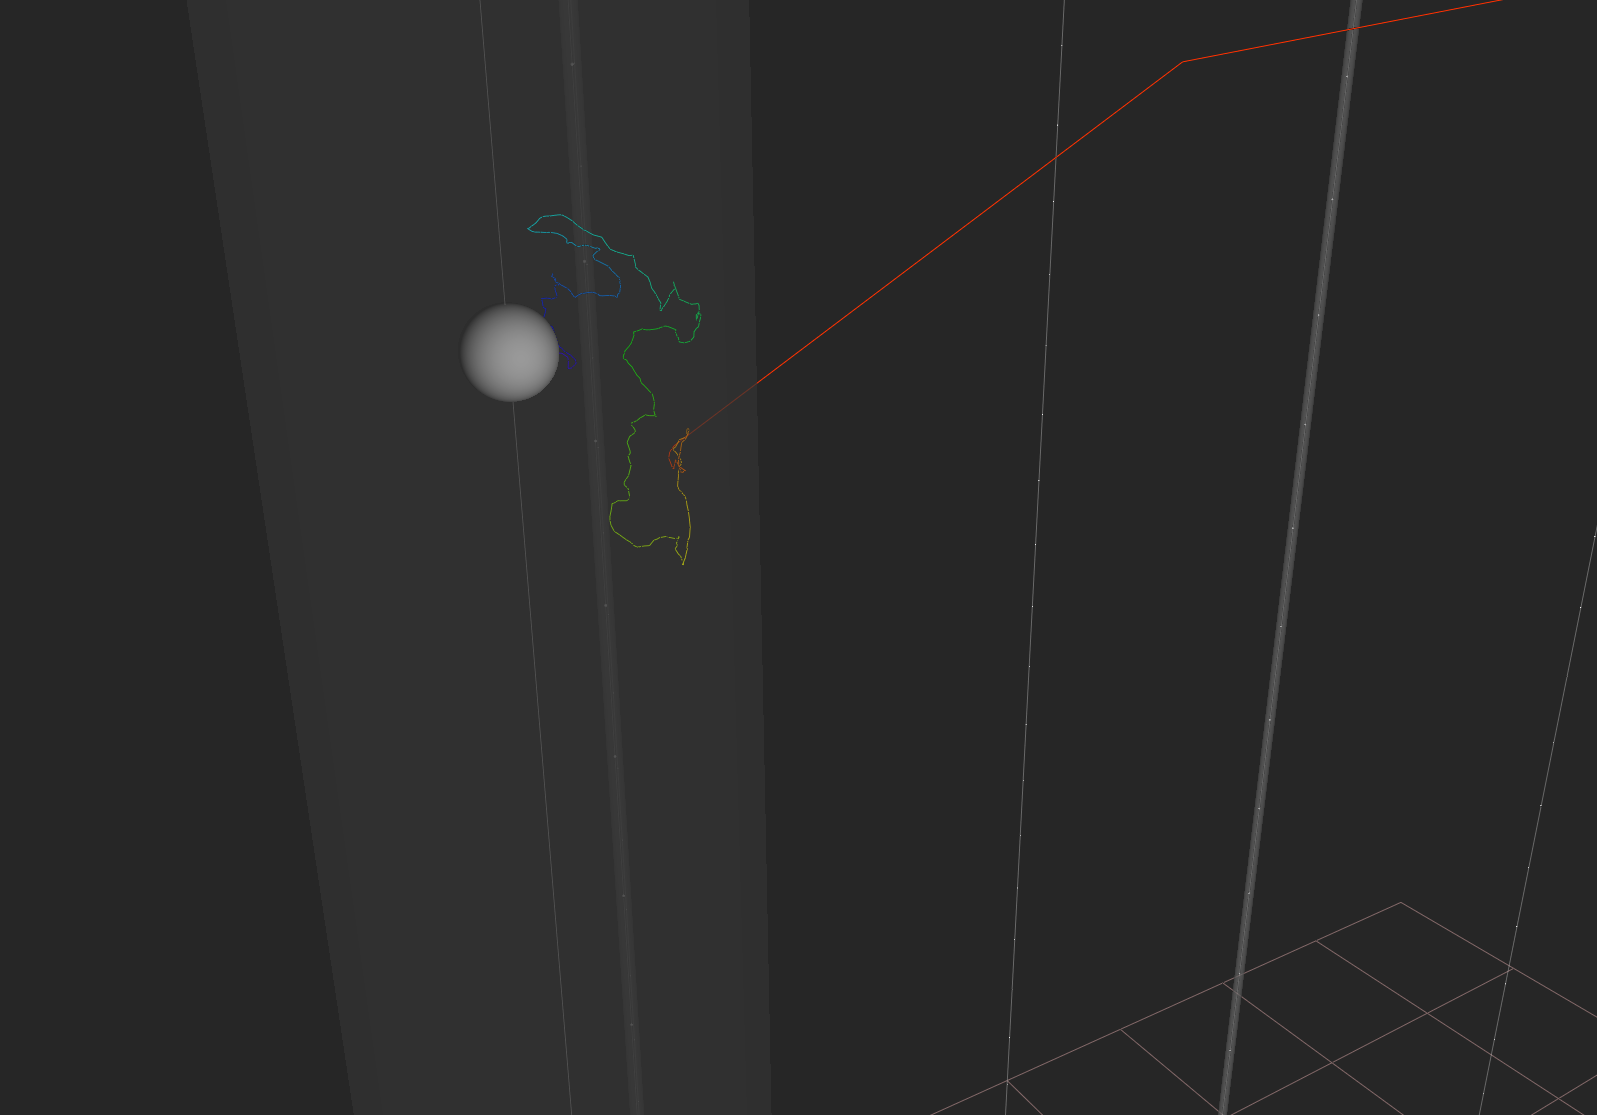
\includegraphics[height=0.35\textheight]{img/flasher-steamshovel-single-received-photon}

  \tiny{See \url{https://github.com/fiedl/hole-ice-study/issues/107}}

\end{frame}
